\tikzstyle{block} = [draw, rectangle, text width=2cm, text centered, minimum height=2cm, node distance=2.7cm]
\tikzstyle{computation-block} = [block, fill=blue!30]
\tikzstyle{memory-block} = [block, fill=green!30]
\tikzstyle{cache-block} = [block, fill=orange!30, minimum height=1cm]

\begin{center}
	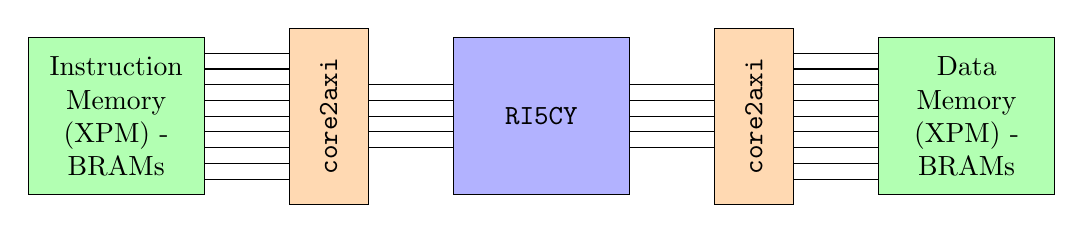
\begin{tikzpicture}
	
	 \node [computation-block] (CPU) {\texttt{RI5CY}};
	 \node [cache-block, right of=CPU, rotate=90] (core2axi-data) {\texttt{core2axi}};
	 \node [cache-block, left of=CPU, rotate=90] (core2axi-inst) {\texttt{core2axi}};
	 \node [memory-block, left of=core2axi-inst] (Imem) {Instruction Memory (XPM) - BRAMs};
	 \node [memory-block, right of=core2axi-data] (Dmem) {Data Memory (XPM) - BRAMs};
	
	\foreach \i in {-2,...,2}{% 
		\draw[-] ([yshift=\i * 0.2 cm]CPU.east) -- ([yshift=\i * 0.2 cm]core2axi-data.north) ;}
	
	\foreach \i in {-2,...,2}{% 
		\draw[-] ([yshift=\i * 0.2 cm]CPU.west) -- ([yshift=\i * 0.2 cm]core2axi-inst.south) ;}
	
	\foreach \i in {-4,...,4}{% 
		\draw[-] ([yshift=\i * 0.2 cm]core2axi-inst.north) -- ([yshift=\i * 0.2 cm]Imem.east) ;}
	
	\foreach \i in {-4,...,4}{% 
		\draw[-] ([yshift=\i * 0.2 cm]core2axi-data.south) -- ([yshift=\i * 0.2 cm]Dmem.west) ;}
	
	\end{tikzpicture}
\end{center}